\documentclass[12pt,a4paper]{article}
\usepackage{tikz}
\usetikzlibrary{arrows.meta,positioning}
\usepackage{tabularx}
\usepackage{graphicx}
\usepackage{amsmath}
\usepackage{amssymb}
\usepackage{amsthm}
\usepackage{bm}
\usepackage{hyperref}
\usepackage{booktabs}
\usepackage{array}
\usepackage{geometry}
\geometry{margin=2.5cm}
\hypersetup{colorlinks=true, linkcolor=blue, citecolor=blue, urlcolor=blue}

\title{\textbf{Paper A-01: Earth Unified Environmental Transport:\\ A Constraint-Driven Flux Dynamics (CDFD) Perspective}}
\author{Steve Bico Mujjabi, MD\\
\small Independent Researcher\\
\small Founder, Vura Labs\\
\small Kampala, Uganda\\
\small ORCID: 0009-0001-0556-5516}
\date{August 2026}

\begin{document}
\maketitle

% BEGIN SHARED-METHODS POINTER
\noindent\textit{Shared Part IV notation and evidence boundaries are defined in \path{PART_IV_METHODS_AND_CLAIM_BOUNDARY.md}. This paper states only its local observables, comparison, and failure conditions.}
% END SHARED-METHODS POINTER

\begin{abstract}
This opening Earth-systems paper states the Part A modelling frame. It treats
environmental transport as a CDFD/AFL hypothesis in which heat, water,
nutrients, sediment, pollutants, and biological energy are represented as
domain-specific fluxes $\Phi$ moving against constraints $C$ through surfaces
with responsiveness $S$ and structural memory $M_s$. The release-local runtime
outputs are internal diagnostics and tests that could break the mapping, not field evidence
of climate, hydrological, ecological, or geological claims.
\end{abstract}

\section{Series Context}

Part I sets the flow--constraint language used here \cite{MujjabiPartI2026}.
Part II develops the Life Number and the origins-of-life use of the same notation
\cite{MujjabiPartII2026}. Part III applies AFL to biology and medicine
\cite{MujjabiPartIII2026}. Part IV \cite{MujjabiPartIV2026}, DOI \url{https://doi.org/10.5281/zenodo.20395901}, uses this Earth-systems opening paper to set
the measurement boundary for the rest of Part A.

\section{Earth-System Transport Frame}

Earth systems are coupled transport networks. Atmospheric circulation moves
heat and moisture; oceans redistribute heat and salinity; rivers move water and
sediment; soils regulate nutrients and organic matter; ecosystems route biomass
and information through trophic structure. CDFD/AFL does not replace the
standard equations in these fields. It supplies a common audit layer for asking
where flow rises, where capacity tightens, where responsiveness is lost, and
where memory keeps a system from returning to its earlier state.

\section{Candidate Variable Map}

\begin{table}[h]
\centering
\begin{tabularx}{\textwidth}{@{}lXX@{}}
\toprule
CDFD term & Earth-system reading & Example proxy \\
\midrule
$\Phi$ & environmental drive or throughput & heat flux, runoff, nutrient load \\
$C$ & active constraint or capacity burden & aridity, channel resistance, toxicity \\
$S$ & responsiveness or buffering & biodiversity, soil structure, wetland storage \\
$M_s$ & structural memory & degradation, hysteresis, legacy contamination \\
$\Psi_s$ & operating ratio & balanced, constrained, or overloaded regime \\
\bottomrule
\end{tabularx}
\end{table}

This map is hypothesis-level until the proxies, scales, datasets, and failure
conditions are specified for a given Earth-system question.

\section{Part A Sequence}

The Part A papers move from broad environmental transport into atmosphere,
ocean, hydrology, soil, ecology, biodiversity, pollution, agriculture,
sustainability, collapse, synthesis, plate tectonics, and volcanology. The
sequence is ordered to start with transport structure, then add specific
environmental constraints and failure modes.

\section{Measurement Layer}

\section{Current Runtime Diagnostic}

The release-local discovery script
includes selected Earth-system adapter rows for climate and atmosphere, ocean
transport, hydrological flow, biodiversity, and pollution. The accompanying
network-cascade diagnostic checks finite-value behavior in an overload and
memory-locking stress test. I use those rows as a runtime audit, not as a
replacement for Earth-system data.

\section{Falsification Targets}

The Earth-systems framing weakens if a domain cannot define measurable
proxies for $\Phi$, $C$, $S$, and $M_s$, if the proposed operating ratio fails
to predict overload or recovery behavior, or if a standard domain model explains
the same data without any added value from the CDFD/AFL mapping.

% BEGIN PART IV MAJOR CROSS-DOMAIN UPGRADE
\section{Cross-Domain Model Upgrade: Mechanism, Scale, and Tests}

\subsection{Observable Translation}

The paper-specific translation begins with an observable chain rather than a
verbal analogy. For Earth Unified Environmental Transport, the proposed drive is radiative, hydrological, biogeochemical, and human forcing.
The active limitation is transport resistance and finite environmental capacity. Responsiveness is carried by
circulation, storage, ecological buffering, and rerouting, while retained state is represented by
soil, ice, ocean, ecological, and contamination legacies. The outcome to explain is redistribution, overload, recovery, and regime change.

\begin{table}[htbp]
\centering
\small
\caption{Operational CDFD/AFL map for Paper A-01.}
\begin{tabularx}{\textwidth}{|l|X|X|}
\hline
\textbf{Term} & \textbf{Paper-specific observable meaning} & \textbf{Measurement question} \\
\hline
$\Phi$ & radiative, hydrological, biogeochemical, and human forcing & What rate, load, gradient, or demand enters the focal system? \\
\hline
$C$ & transport resistance and finite environmental capacity & Which measured bottleneck limits transfer, function, or recovery? \\
\hline
$S$ & circulation, storage, ecological buffering, and rerouting & Which process changes effective capacity or reroutes the load? \\
\hline
$M_s$ & soil, ice, ocean, ecological, and contamination legacies & Which retained state makes equal present loads produce different futures? \\
\hline
$Y$ & redistribution, overload, recovery, and regime change & Which outcome is predicted out of sample, with uncertainty? \\
\hline
\end{tabularx}
\end{table}

\begin{figure}[htbp]
\centering
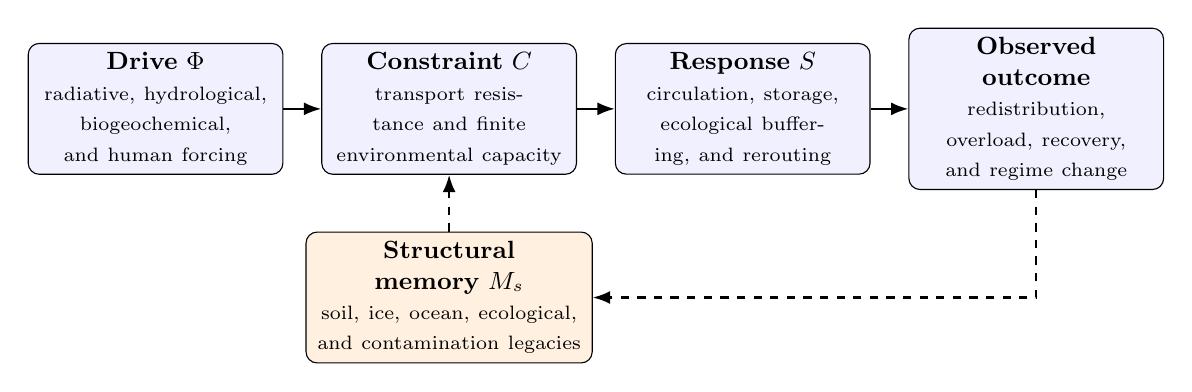
\begin{tikzpicture}[
    node distance=0.48cm,
    every node/.style={font=\small},
    box/.style={draw, rounded corners, align=center, minimum height=1.45cm, text width=3.0cm, fill=blue!6},
    memory/.style={draw, rounded corners, align=center, minimum height=1.25cm, text width=3.4cm, fill=orange!12},
    flow/.style={-{Latex[length=2.2mm]}, thick},
    feedback/.style={-{Latex[length=2.2mm]}, thick, dashed}
]
\node[box] (drive) {\textbf{Drive $\Phi$}\\\scriptsize radiative, hydrological, biogeochemical, and human forcing};
\node[box, right=of drive] (constraint) {\textbf{Constraint $C$}\\\scriptsize transport resistance and finite environmental capacity};
\node[box, right=of constraint] (response) {\textbf{Response $S$}\\\scriptsize circulation, storage, ecological buffering, and rerouting};
\node[box, right=of response] (outcome) {\textbf{Observed outcome}\\\scriptsize redistribution, overload, recovery, and regime change};
\node[memory, below=0.72cm of constraint] (memory) {\textbf{Structural memory $M_s$}\\\scriptsize soil, ice, ocean, ecological, and contamination legacies};
\draw[flow] (drive) -- (constraint);
\draw[flow] (constraint) -- (response);
\draw[flow] (response) -- (outcome);
\draw[feedback] (outcome.south) |- (memory.east);
\draw[feedback] (memory.north) -- (constraint.south);
\end{tikzpicture}
\caption{Paper A-01 observable CDFD/AFL architecture for Earth Unified Environmental Transport. Solid arrows give the proposed forward chain; dashed arrows make history-dependent feedback explicit.}
\label{fig:a01-architecture}
\end{figure}

\subsection{Paper-Specific Causal Hypothesis}

For this paper, the hypothesized causal sequence is specific. A change in
radiative, hydrological, biogeochemical, and human forcing arrives faster than circulation, storage, ecological buffering, and rerouting can compensate.
This raises or redistributes transport resistance and finite environmental capacity. If the load persists,
the retained state encoded by soil, ice, ocean, ecological, and contamination legacies changes the next response, so a later event of equal
magnitude can produce a different trajectory in redistribution, overload, recovery, and regime change. The
scientific task is to estimate that sequence against the best ordinary model of
the domain, not merely to redescribe the outcome after it occurs.

\subsection{Cross-Scale Translation Without Mechanistic Erasure}

For the Earth systems family, the cross-domain translation compares coupled transport, finite environmental capacity, buffering, and retained landscape or ecosystem state. It cannot erase conservation laws, geometry, or scale; it must expose where those domain equations create comparable overload and recovery structures. \cite{Holling1973,Turing1952,BakTangWiesenfeld1987}
The required scale declaration for this paper is hours to millennia; catchments to the coupled Earth system. At short
scales, the key question is whether the incoming drive is transmitted,
buffered, or diverted. At intermediate scales, response changes effective
capacity and network exposure. At long scales, retained structure can alter the
state space itself. A result is genuinely cross-scale only when the aggregation
rule is stated and the same conclusion is not an artifact of averaging.

\subsection{Evidence Ladder and Discriminating Tests}

\begin{table}[htbp]
\centering
\small
\caption{Evidence ladder for Paper A-01. Each rung can fail independently.}
\begin{tabularx}{\textwidth}{|p{0.17\textwidth}|X|X|}
\hline
\textbf{Test} & \textbf{Design} & \textbf{Discriminating result} \\
\hline
Proxy audit & Measure coupled reanalysis, remote sensing, gauge records, and ecological time series and preregister how each record maps to $\Phi$, $C$, $S$, $M_s$, and $Y$. & The mapping fails if proxies are non-identifiable, circular, or change meaning across cases. \\
\hline
Load ramp & Apply or observe a compound heat, rainfall, and pollutant pulse while estimating the dominant constraint and response time. & A threshold claim requires a reproducible nonlinear change and uncertainty bounds, not a visually chosen breakpoint. \\
\hline
Recovery and memory & Match present load across units with different histories, then compare recovery paths. & The memory claim requires history-dependent divergence after current conditions are controlled. \\
\hline
Model comparison & Compare the baseline domain model with and without the CDFD/AFL state variables using held-out data. & The paper's stated falsifier is: the added variables do not improve prediction beyond ordinary coupled transport budgets. \\
\hline
\end{tabularx}
\end{table}

\subsection{Research Programme and Boundary Conditions}

The immediate research programme has four steps. First, construct a documented
dataset from coupled reanalysis, remote sensing, gauge records, and ecological time series and retain raw units before normalization.
Second, fit a baseline domain model and report its calibration and out-of-sample
error. Third, add the smallest identifiable CDFD/AFL state extension and test
whether it improves prediction of redistribution, overload, recovery, and regime change. Fourth, repeat the
analysis across the declared scale range and publish negative cases as part of
the cross-domain translation audit.

% END PART IV MAJOR CROSS-DOMAIN UPGRADE

\section{Conclusion}

Part A uses CDFD/AFL as a shared transport language for Earth systems. The
framework is useful only when it sharpens measurable hypotheses and failure
conditions. It remains separate from operational climate, hydrological,
ecological, agricultural, or geological advice.

\section*{Conflict of Interest}
The author declares no conflict of interest.

\section*{Data Availability}
Part-specific runtime diagnostics are under each Part's \path{outputs/} directory.

Release-wide code: \path{Part_E_Synthesis/supplementary/}.

Generated summaries: \path{Part_E_Synthesis/outputs/}.

Figures: \path{Part_E_Synthesis/figures/}.


\section{Reference Layer}
\bibliographystyle{plain}
\bibliography{universal_afl_references}
\end{document}
